\begin{figure}[H]
  \centering
  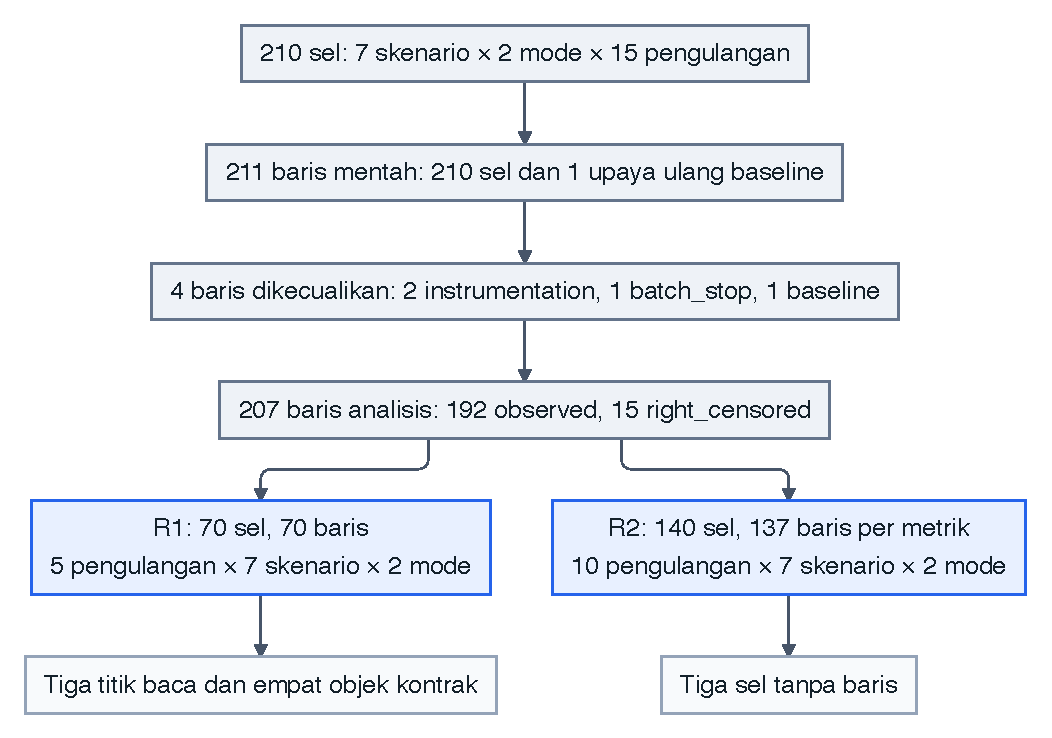
\includegraphics[width=\textwidth]{diagrams/fig-analysis-flow.pdf}
  \caption{Alur analisis dari 210 sel dan 211 baris mentah, empat baris yang dikecualikan, 207 baris analisis, lalu jalur waktu RQ (140 sel, 137 baris per metrik) dan kotak validitas R1 (70 sel, 70 baris), dengan anotasi kasus batas G. Titik akhir dapat lengkap, tersensor, atau tidak teramati sebelum berhenti.}
  \label{fig:alur-analisis}
\end{figure}
